\section{Week 3 - Discreete Random Vars}
\subsection{Random Variable - Informal Definitions}
A random variable X (or some other upper case letter ) is a variable that takes a numerical value x (lower case), which depends on a random experiment.
The values depend on outcomes of a random phenomenon.\\
\textbf{Discreete:} X takes any of a finite set of values, e.g. {1.5, 2.693, 5, 6.3, 10}\\
\textbf{Continuous:} X takes any value of an uncountable range, e.g. the real numbers in the interval (2, 7)).\\
Before observing the outcome of a random experiment, the ``best we can know'' is a list of all possible values, and a list for each possible value how likely it will occur.
\subsubsection{Other definitions}
\textbf{Algebra:} variable value turns the equation into a true (not changeable)\\
\textbf{Programming:} variable value is determined (and changeable) by the assignment.

\subsubsection{Example}
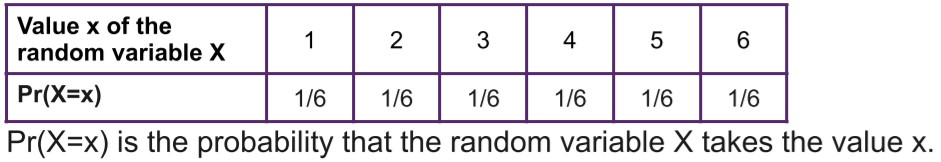
\includegraphics[width=\linewidth]{discreete-var_example.jpg}
\textbf{Probability Mass Function:}
A PMF specifies a (discrete) Probability Distribution.\\
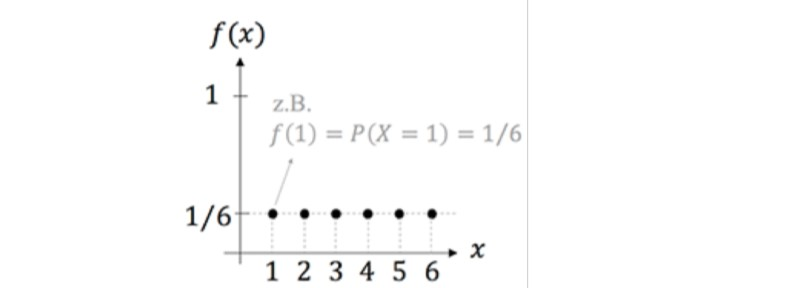
\includegraphics[width=\linewidth]{pmf.jpg}

\subsection{Joint-Probability}
This is usually written as \textbf{Pr(X=5, Y=4) = 1/36} or more compact as \textbf{p(5,4)=1/36} you'll also come across \textbf{PXY (5,4)=1/36}
The komma is a logical \textbf{AND}.\\
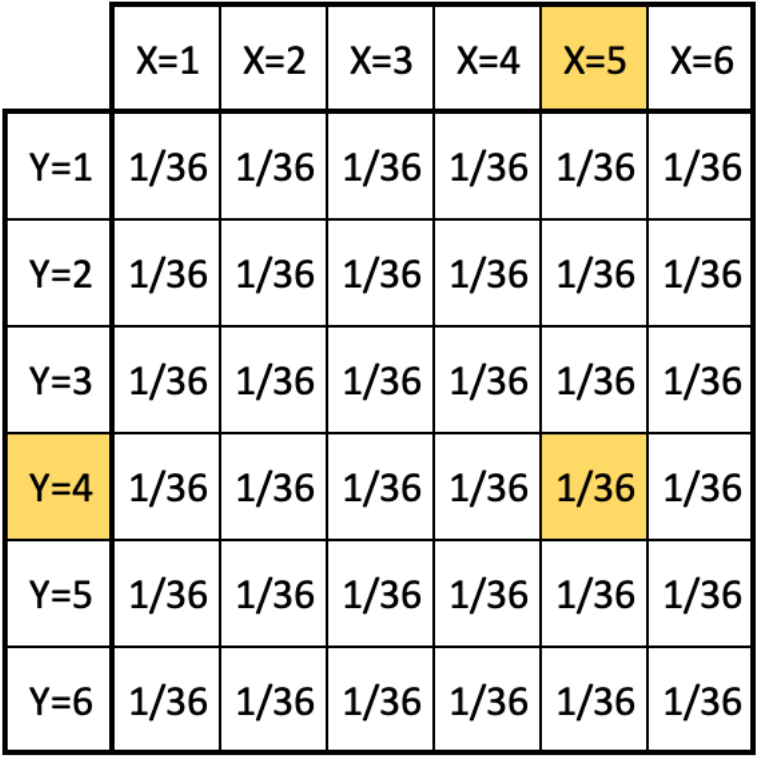
\includegraphics[width=\linewidth]{joint-probability.png}

\subsubsection{Marginal Probability}
Marginal probability is the probability of an event irrespective of the outcome of another variable.
Can be calculated from the Joint Probability. (Spalte von Joint Probability)

\subsection{Independent random variables}
If the first dice is a 6, there is no probability that the second dice is also a 6.
If X and Y are independent:\\
Pr(X,Y) = Pr(X) * Pr(Y)

\subsection{Correlated random variables}
Events that are \textbf{not independent.}\\
Here given as joint probability:\\

\includegraphics[width=\linewidth]{joint-probability.jpg}
X: The event to observe clouds ( 0= no clouds, 1= small clouds, 2= big clouds)\\
Y: The event that it rains ( 0=no rain, 1=light rain, 2=moderate rain, 3=heavy rain)

\subsubsection{Conditional Probability}
Consider: You observe small clouds. What is the probability for moderate rain?
The observation X is no longer random. X is observed, its value is fixed. We say ``X is given''.
To answer the question, we calculate the probabilities of Y given X with \textbf{Pr(Y|X)}.\\
\textbf{Important:} Do not just read the 0.05 in this example, because the total value of the Column is \textbf{not 1.}\\
\textbf{P(Y|X) = P(X,Y) / P(X)}\\
In this example: P(Y|X) = 0.05 / 0.35 = 0.1428 = 14.28\%

\subsection{Bayes Rule}
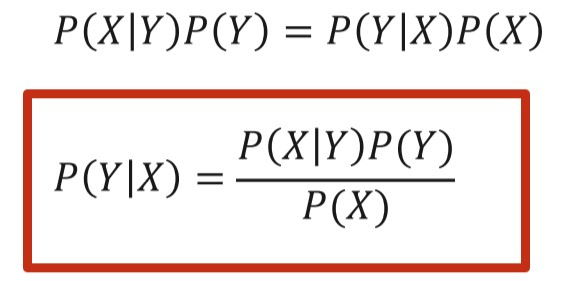
\includegraphics[width=\linewidth]{bayes.jpg}

\subsection{Empirical rule}
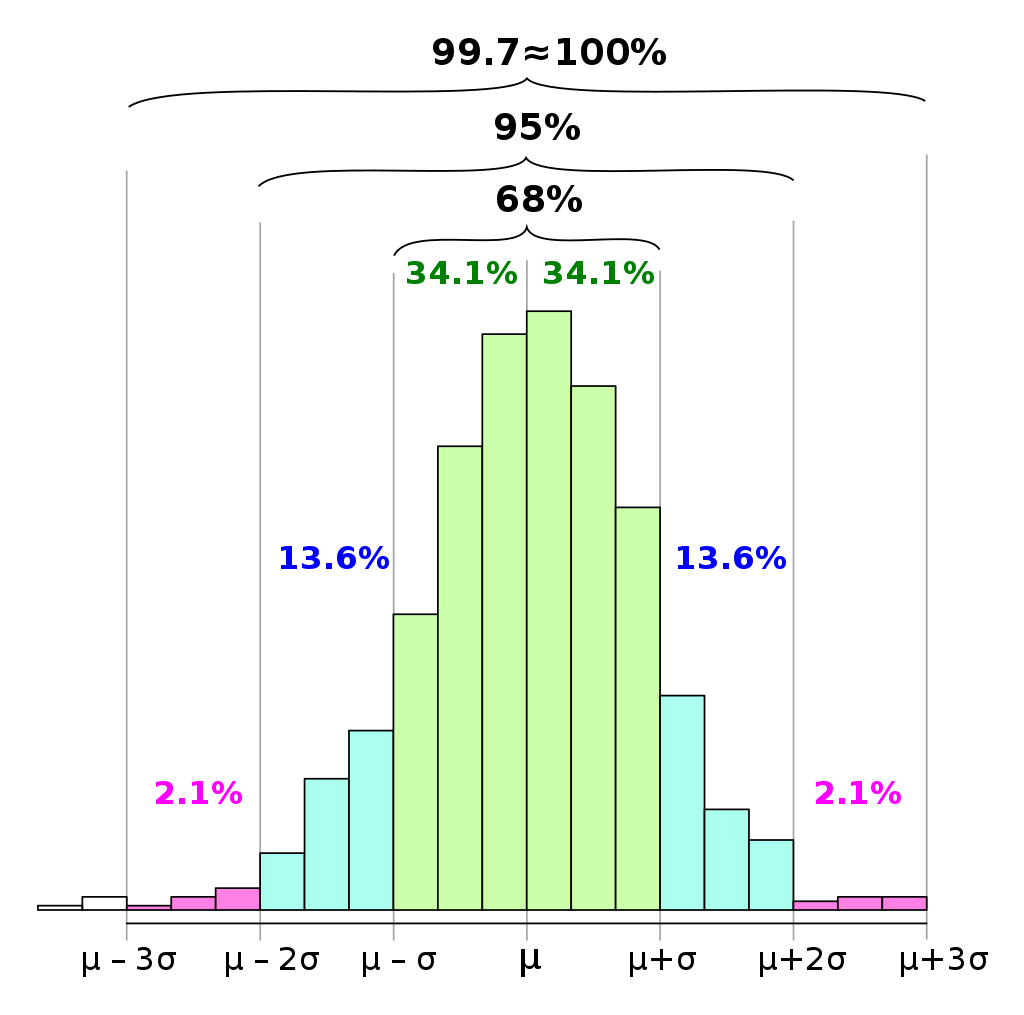
\includegraphics[width=\linewidth]{empirical-rule.png}